\documentclass[border=8pt]{standalone}
\usepackage{tikz}
\usetikzlibrary{arrows.meta,positioning,calc}
\begin{document}
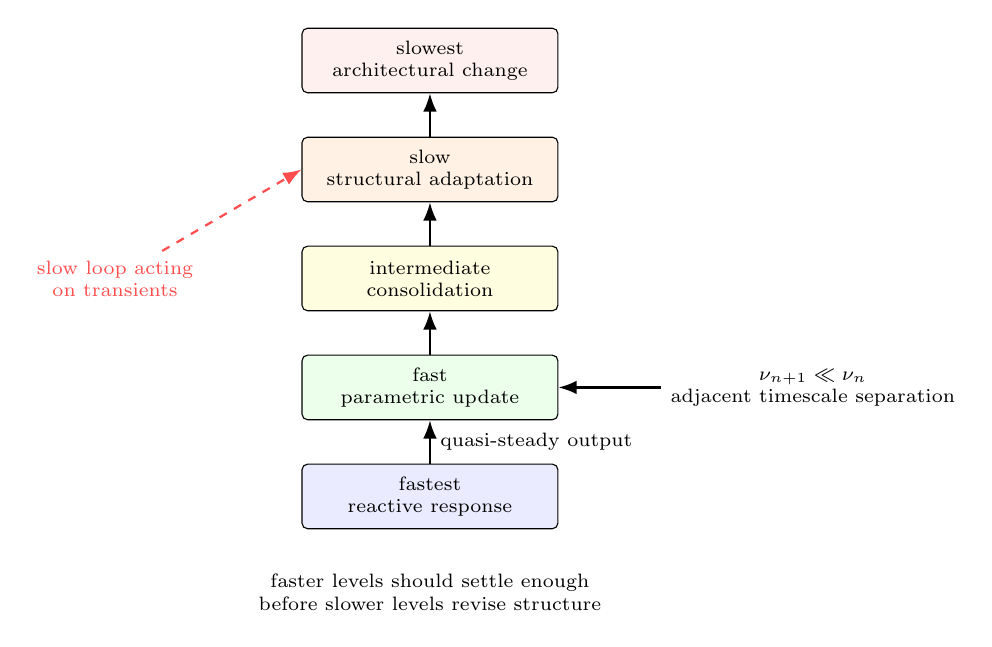
\begin{tikzpicture}[
  box/.style={draw, rounded corners=2pt, align=center, minimum width=3.25cm, minimum height=0.82cm, font=\scriptsize},
  note/.style={align=center, font=\scriptsize},
  arr/.style={-Latex, thick},
  warnarr/.style={-Latex, thick, dashed, red!70}
]

\node[box, fill=red!6] (arch) {slowest\\architectural change};
\node[box, fill=orange!10, below=0.55cm of arch] (struct) {slow\\structural adaptation};
\node[box, fill=yellow!12, below=0.55cm of struct] (consol) {intermediate\\consolidation};
\node[box, fill=green!8, below=0.55cm of consol] (param) {fast\\parametric update};
\node[box, fill=blue!8, below=0.55cm of param] (react) {fastest\\reactive response};

\draw[arr] (react) -- node[right, font=\scriptsize] {quasi-steady output} (param);
\draw[arr] (param) -- (consol);
\draw[arr] (consol) -- (struct);
\draw[arr] (struct) -- (arch);

\node[note, right=1.3cm of param] (ratio) {$\nu_{n+1}\ll\nu_n$\\adjacent timescale separation};
\draw[arr] (ratio) -- (param);

\node[note, left=1.25cm of consol, text=red!70] (osc) {slow loop acting\\on transients};
\draw[warnarr] (osc) -- (struct.west);
\node[note, below=0.45cm of react] {faster levels should settle enough\\before slower levels revise structure};

\end{tikzpicture}
\end{document}
